% Created 2011-08-25 Thu 13:07
\documentclass[10pt,english]{article}
\usepackage[utf8]{inputenc}
\usepackage[T1]{fontenc}
\usepackage{fixltx2e}
\usepackage{graphicx}
\usepackage{longtable}
\usepackage{float}
\usepackage{wrapfig}
\usepackage{soul}
\usepackage{textcomp}
\usepackage{marvosym}
\usepackage{wasysym}
\usepackage{latexsym}
\usepackage{amssymb}
\usepackage{hyperref}
\tolerance=1000
\usepackage{color}
\usepackage{listings}

\usepackage{lmodern}
\renewcommand{\sfdefault}{lmss}
\renewcommand{\ttdefault}{lmtt}

% needed packages
\usepackage{amsmath}
\usepackage{amssymb}
\usepackage{amsthm}
\usepackage{babel}
\usepackage{epsfig}
\usepackage[T1]{fontenc}
\usepackage{fixltx2e}
\usepackage{float}
%\usepackage{floatflt}
\usepackage{graphics}
\usepackage{graphicx}
\usepackage[utf8]{inputenc}
\usepackage{latexsym}
\usepackage{longtable}
\usepackage{makeidx}
\usepackage{marvosym}
\usepackage{multicol}
%\usepackage{pslatex}
\usepackage{rotating}
%\usepackage{showidx}
\usepackage{soul}
\usepackage{srcltx}
\usepackage{stmaryrd}
\usepackage{subfig}
\usepackage{textcomp}
%\usepackage{theorem}
%\usepackage[subfigure]{tocloft}
\usepackage{txfonts}
\usepackage{upgreek}
\usepackage{url}
\usepackage{varioref}
%\usepackage{wasysym}
\usepackage{wrapfig}


% Page setup
\usepackage[paperwidth=8.5in,paperheight=11in]{geometry}
\geometry{verbose,tmargin=0.5in,bmargin=0.5in,lmargin=1in,rmargin=1in}




% PDF settings
%\usepackage[hyperref,x11names]{xcolor}
\usepackage{hyperref}
\hypersetup{pdftitle={STAT 5840: Statistical Computing},
 		pdfauthor={G. Jay Kerns}, 
		linkcolor=Firebrick4, 
		citecolor=black, 
		urlcolor=SteelBlue4}

% Listings setup
%\usepackage{color}
%\usepackage{listings}
%\lstset{basicstyle={\ttfamily},
%	language=R,
%	breaklines=true,
%	breakatwhitespace=true,
%	keywordstyle={\ttfamily},
%	numberstyle = {\ttfamily},
%	morestring=[b]"
%}



%  user defined commands
% special operators
\renewcommand{\P}{\mathrm{I\hspace{-1.5pt}P}}
\newcommand{\E}{\mathrm{I\hspace{-1.5pt}E}}
\renewcommand{\vec}[1]{\mbox{\boldmath$#1$}}

% special symbols
\newcommand{\me}{\mathrm{e}}
\newcommand{\R}{\mathbb{R}}
\newcommand{\diff}{\mathrm{d}}
\newcommand{\ybar}{\overline{y}}
\newcommand{\xbar}{\overline{x}}
\newcommand{\Xbar}{\overline{X}}
\newcommand{\Ybar}{\overline{Y}}





\providecommand{\alert}[1]{\textbf{#1}}

\title{STAT 5840 | Statistical Computing | Introduction to \texttt{R}}
%\author{G. Jay Kerns}
\date{}

\begin{document}

\maketitle

\thispagestyle{empty}

\section*{Illustration of the basic Monte Carlo method: \textbf{estimating areas}.}
\label{sec-1}



\begin{enumerate}
\item We will usually write programs (or ``scripts'') and save them on the Desktop (or some other folder of your choice).  For this lab it may make your life easier to download the \texttt{IntroRinclass.R} script and work from there.
\item We would like to estimate the area of a region $E$ inside the unit square.

   \begin{center}


   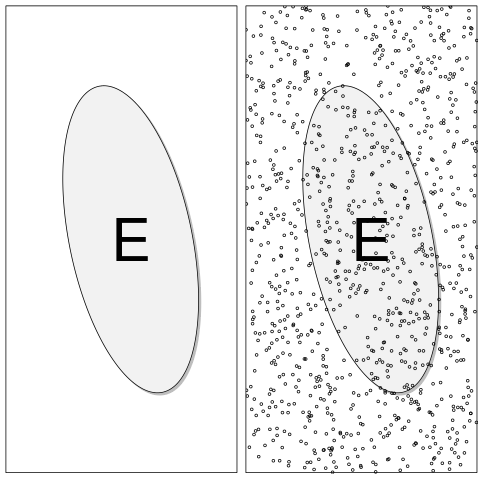
\includegraphics[width=3in, height=1.5in,]{img/IntroR.pdf}

   \end{center}

   Suppose we can generate a pair \( (x,y) \) of random numbers, each chosen independently at random from [0,1].  Then \( (x,y) \) are the coordinates of a point chosen at random from the unit square.  If we would like to estimate the area of the region, we could choose a large number of random points and record the fraction that fall in the region.

   \textbf{Example:} $E = \{ (x,y)\, : \, y \leq x^2  \}$.
\end{enumerate}


\begin{verbatim}
   # IntroRinclass.R

   Iter <- 1000; count <- 0           # initialization and storage
   for (i in 1:Iter){                 # start the simulation loop       
     x <- runif(1); y <- runif(1)     # generates two rand coords
     if (y <= x^2){ 
       count <- count + 1             # accept the point
     }
   }
   accept <- count/Iter               # store prop of accepts
   accept                             # print prop of accepts
   sqrt(accept*(1-accept)/Iter)       # print std error of estimate
\end{verbatim}




\begin{verbatim}
    [1] 0.336
    [1] 0.01493667
\end{verbatim}



\begin{enumerate}
\item For each of the following, find 1) an estimate of the area, 2) an error of estimate, and 3) the exact value.
\begin{enumerate}
\item \( E = \{ (x,y) : y > |\sin(5 \pi x)| \} \).
\item \( E = \{ (x,y) : y < 1024 x^5 (1-x)^5 \} \).
\item \( E = \{ \mbox{inside circle with center (0.5,0.5) and radius 0.5}\} \).
\end{enumerate}
\end{enumerate}
\textbf{Hints:}

\begin{itemize}
\item the \texttt{R} functions for absolute value and sine are \texttt{abs} and \texttt{sin}, respectively (and $\pi$ is just \texttt{pi}).
\item the equation of a circle with center \( (a,b) \) and radius $r$ is \( (x-a)^{2} + (y-b)^{2} = r^{2} \).
\item you can open a new \texttt{R} script with File, New, R Script, and you can open an existing script with File, Open File\ldots{}
\end{itemize}

\end{document}